% !TeX root = ./main.tex
\documentclass{iiitkthesis}

%-----------------------------------------
% Packages
%-----------------------------------------
\usepackage{graphics} % for pdf, bitmapped graphics files
\usepackage{epsfig} % for postscript graphics files
\usepackage{amsmath} % assumes amsmath package installed
\usepackage{cite}
\usepackage{color}
\usepackage{colortbl}
\usepackage{tcolorbox}
\usepackage{adjustbox}
\usepackage{multirow}
\usepackage{pgfplots}
\usepackage{csquotes}
\usepackage[linesnumbered,algoruled,boxed,lined]{algorithm2e}
\usepackage{textcomp}
\usepackage[T1]{fontenc}
\usepackage{varioref}
\usepackage{float}
\usepackage{epstopdf} % To use .eps images
\usepackage{times}
\usepackage[section]{placeins} % to keep floats(figures) in the section in which they were issued
\usepackage{amssymb}
\usepackage{url}
\usepackage{subfig}
\usepackage{textcomp}
\usepackage{sidecap}
\usepackage{verbatim} %%% for clock comments 
\usepackage{amsthm}
\usepackage{listings}
\usepackage{color} %red, green, blue, yellow, cyan, magenta, black, white
\usepackage{hyperref}

%-----------------------------------------
% Start of the document
%-----------------------------------------

\begin {document}

%-----------------------------------------
% Title page
%-----------------------------------------

\begin{titlepage}
    \begin{center}
        {\Large  \bfseries OCR of Offline Hindi Handwritten Text}\\

        \vfill
        B. Tech Major Project\\

        \vfill
        By:-\\
        Raghav Jajoo --- 2019KUCP1082\\
        Rishabh Chauhan --- 2019KUCP1071\\
        Ayush Kumar Mohanta --- 2019KUCP1033\\

        \vfill
        Mentor: Dr. Basant Agarwal\\

        \vfill
        \begin{figure}[h]
            \centering
            
\includegraphics[width=40mm]{figures/IIITKota.png}
        \end{figure}

        \vfill
        Computer science and Engineering\\
        \textbf{INDIAN INSTITUTE OF INFORMATION TECHNOLOGY KOTA}\\
        MNIT Campus, Jaipur, INDIA.\\
        2021-2022

    \end{center}
\end{titlepage}
  
%-----------------------------------------
% Declaration and acknowledgement
%-----------------------------------------

\chapter*{DECLARATION}
\thispagestyle{empty}

\doublespace

\qquad 

\indent I hereby {\textit{declare}} that the Major Project entitled {\bf \textquotedblleft{OCR of offline Hindi handwritten text\textquotedblright}}, which is being submitted to the {\bf\textit{Indian Institute of Information Technology Kota}} in partial fulfilment of the requirements for the award of the Degree of {\bf\textit{Bachelor of Technology-CSE}} in {\bf\textit{Raghav Jajoo, Ayush Kumar Mohanta and Rishabh Chouhan}} is a {\textit{bonafide report of the Project work carried out by me}}. The material contained in this thesis has not been submitted to any University or Institution for the award of any degree.

\vspace*{1in}
\begin{singlespace}
\hspace*{1.5in} 
\parbox{3in}
{{\noindent { Raghav Jajoo — 2019KUCP1082}}\\
{\noindent { Rishabh Chauhan — 2019KUCP1071}}\\
{\noindent { Ayush Kumar Mohanta — 2019KUCP1033}}\\
\noindent {Computer Science and Education}\\
\noindent {Indian Institute of Information Technology Kota}}
\end{singlespace} 

\vspace*{1in}

\noindent Place: IIIT Kota, Jaipur\\
\noindent Date: \today 
\par\newpage


\chapter*{CERTIFICATE}
\thispagestyle{empty}

\doublespace

\qquad 

\vspace*{0.5in}
\indent This is to \textit{certify} that the Research Thesis entitled {\bf \textquotedblleft{OCR of offline Hindi handwritten text \textquotedblright}}, submitted by {\bf Raghav Jajoo, Rishabh chouhan and Ayush kumar mohanta} as the record of the research work carried out by him, is \textit{accepted} as the \textit{Research Thesis submission} in partial fulfillment of the requirements for the degree of {\bf\textit{B. Tech}}.

\vspace*{1in}

\begin{singlespace}
\hspace*{1.5in} 
\parbox{3in}
{\noindent {\bf Dr Basant Agarwal} \\
\noindent Research Guide \\ 
\noindent Professor\\
\noindent Computer Science and Engineering\\
\noindent IIIT Kota }

\end{singlespace} 
\vspace*{0.25in}
\par\newpage

%-----------------------------------------
% Abstract
%-----------------------------------------

\begin{abstract}
    \thispagestyle{empty}
    
    Optical Character Recognition is a system which can perform the translation of images from handwritten or printed form to machine-editable form.
    OCR converts normal scanned documents text-searchable so to allow content search on the same. Hindi being the national language of India, with such huge population makes document managing and preservation difficult in government sector. Hence, this paper presents an efficient algorithm CRNN and CTC for recognition of Hindi script characters from printed documents.
    One of the major reasons for the poor recognition rate is error in character segmentation. The presence of touching characters in the scanned documents further complicates the segmentation process, creating a major problem when designing an effective character segmentation technique. Preprocessing, character segmentation, feature extraction, and finally, recognition are the major steps which are followed by a general OCR.
    
    Keywords - OCR, CRNN, CTC, Preprocessing, character segmentation, Feture Extraction, Recognition.
\end{abstract}

%-----------------------------------------
% Table of con, list of figures and tables
%-----------------------------------------

\tableofcontents

%-----------------------------------------
% Chapters
%-----------------------------------------

\chapter{Introduction}
\label{intro}

Optical Character Recognition abbreviated as OCR is the electronic translation of images of handwritten, typewritten or printed text into a machine editable text. An OCR system enables you to take a book or magazine article, feed it directly into an electronic computer file, and then edit the generated text file using a word processor. Thus it can convert the printed characters on the scanned page into editable text. OCR is a field of research which comes under the area of pattern recognition and artificial intelligence. OCR converts printed or handwritten scanned documents into ASCII characters that a computer can recognize.
\section{Problems in OCR:-}
\begin{itemize}
\item Non-Latin language advancements have been slow. 
\item Lack of data
\item Different styles and inconsistent way of writing
\end{itemize}

\section{Uses of OCR:-}
\begin{itemize}
\item Authentication of signatures in banks
\item Processing of archived institutional records
\item Recognizing ZIP code addresses on letters
\end{itemize}

\chapter{Working in Hindi}
\label{chap:hindi}

Devanagari script is the script for writing Hindi language. Hindi is the official language of India. Hindi is spoken in almost all of India. It includes 13 vowels and 36 consonants. Apart from this, it has basic 11 modifiers which are combined with different consonants and vowels.

Each vowel except the first one has a corresponding modifier using which we can modify a consonant. This line which is available on the upper side of a character is called “Shirorekha''. Based on this shirorekha each character is divided into three distinct parts. The portion in the upper side of shirorekha is called upper modifiers, in the middle portion the character is available and in the last portion lower modifiers are available. 
\subsubsection{The major problems with this script which require special attention are:}
\begin{enumerate}
\item “Shirorekha” or the header line above each and every character.
\item Attachment of modifiers before, after, above, below and within the base vowels and consonants.
\item Large number of symbols
\item Joint, touching and broken characters
\end{enumerate}
\chapter{Processes of OCR}
\label{ch:tech_stuff}

%-----------------------------------------
% Sections
%-----------------------------------------

The algorithm that is used to develop the OCR software for printed Hindi characters is based on the different geometrical features/shapes of Hindi characters. Input image is parsed into many sub parts/images based on these features. Then other properties such as distribution of points/pixels and edges within each sub image are features used to recognize parsed symbols.

There are mainly four steps performed in any OCR system:- 
\begin{enumerate}
\item Pre Processing 
\item Segmentation 
\item Character Recognition 
\item Post Processing.
\end{enumerate}

\section{Pre Processing}
The pre-processing phase includes the steps that are necessary to bring the input data into an acceptable form for the further phases. The steps are: 
\begin{enumerate}
\item RGB to GRAY
\item Binarization 
\item Noise removal and smoothing 
\item Skew detection and correction
\end{enumerate}

\subsection{GrayScale Conversion}
In the first process, The input is converted in a gray scale image. A gray scale image is an image having BW shades. The image is converted into a grayscale image to further convert it into an BW image. Gray image has shades from black to white.

\subsection{Binarization}
Since the developed system is only able to perform its task only on binarized images, we have to perform the binarization operation before the actual task starts.
Basically in binarization, all the pixels above the threshold value are assigned a particular value for instance 1 and all the values below the threshold value are given the value = 0.
\subsubsection{There are different types of thresholding for binarization:-}
\begin{itemize}
\item Simple thresholding.
\item Otsu's Binarization.
\end{itemize}

\subsection{Smoothing and noise removal:-}
Images do have some stray pixels and some unwanted marks. By using filter noise can be filtered from the image. Smoothing operation in gray image is used for noise reduction and filtering is used for noise removal. Basically there are two types of filters, linear filter and order statistics filter. Order statistics filters are non-linear filters whose response is based on the ranking of the pixel and then replacing the value of the center pixel with the value known by ranking result. The best example of a non-linear filter is a median filter.

\subsubsection{Median Filtering:-}
The median filter is a non-linear digital filtering technique, often used to remove noise from an image. Such noise reduction is a typical pre-processing step to improve the results of the later processing. This is highly effective in removing salt-and-pepper noise.

\subsection{Skew detection and correction:-}
The deviation of the baseline of the text is called skew. During the scanning process, the whole document or a portion of it is fed through the scanner. Our main goal during skewing will be splitting the rotated image into text blocks, and determining the angle from them. We here create two functions, one of determining the skew angle and the other of rotating the image.

What we are trying to do here is to create bounding boxes around the text and then choosing the largest bounding box and then determining the skew angle from the box. The process at first involves finding the areas of text. To make text block detection easier we will invert and maximize the colors of our image, that will be achieved via thresholding. 

\begin{figure}[H]
    \centering
    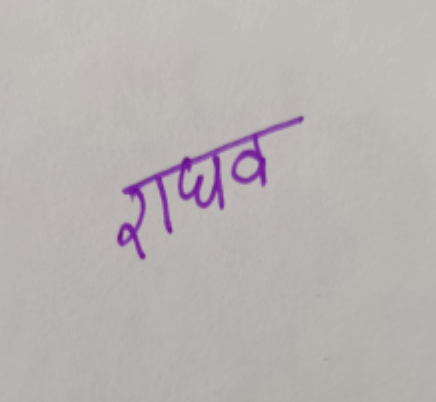
\includegraphics[width=50mm]{figures/image1.png}
    \caption{Before Pre processing}
\end{figure}

\begin{figure}[H]
    \centering
    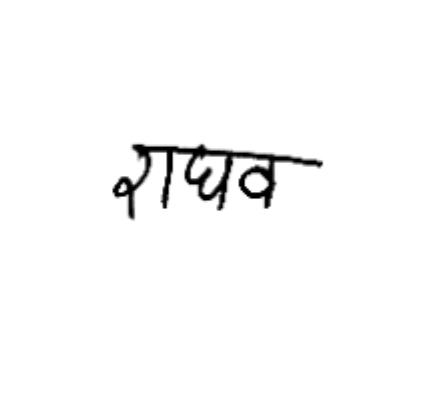
\includegraphics[width=50mm]{figures/image2.png}
    \caption{After Pre processing}
\end{figure}

\newpage

\section{Segmentation}
Segmentation is the way toward parceling a picture/record into disjoint and homogeneous areas. Segmentation is one of the most significant and fundamental procedures that improve the precision pace of character recognition framework. Devanagari report is apportioned into grouping of lines and words by vertical and even projection separately. Process of segmentation involves:-
\begin{enumerate}
\item Segmentation of lines
\item Segmentation of words 
\item Segmentation of characters 
\end{enumerate}

\subsection{Segmentation of lines}
\begin{itemize}
\item A horizontal scanning method is applied for segmenting the text paragraphs into lines. 
\item While performing the segmentation to extract the lines from the text blocks, it performs horizontal scanning starting from the top of the scanned document till it locates the last row containing all white pixels, before a black pixel row is encountered. 
\item It continues the scanning further, till it locates the first row containing all white pixels, just after the end of the last row of black pixels. 
\item This determines a line, and is eventually extracted. This whole process is repeated on the entire text page to segment all the text lines present in that particular page/paragraph.
\end{itemize}

\subsection{Segmentation of Words}
\begin{itemize}
\item After segmenting the lines it segments the individual words embedded in each line.
\item To perform this operation a vertical scanning method is applied. The vertical scanning is applied to the width of the line only. 
\item Analysis of this projection will give us a clear idea about the starting and ending column of each character lying within that text line and amount of space between two adjacent characters.
\end{itemize}

\subsection{Segmentation of Characters}
\begin{itemize}
\item A further segmentation process is applied to achieve the individual characters out of the segmented words. 
\item Before segmenting words at character level, the header line or shirorekha is identified and removed. 
\item Once the shirorekha is properly removed, the word is divided into three horizontal zones known as upper, middle and lower zones. Individual characters are separated from each zone by applying vertical scanning
\end{itemize}


\section{Character Recognition}
After the extraction of individual characters occurs, a recognition engine is used to identify the corresponding computer character. Several different recognition techniques are currently available.

\subsection{K-Nearest Neighbor(KNN) Algorithm for Machine Learning:-}
\begin{itemize}
\item K-Nearest Neighbour is one of the simplest Machine Learning algorithms based on Supervised Learning technique.
\item The K-NN algorithm assumes the similarity between the new case/data and available cases and puts the new case into the category that is most similar to the available categories.
\item KNN algorithm is used for classification (most commonly) and regression. It is a versatile algorithm also used for imputing missing values and resampling datasets.
\item There are three limitations of KNN:-
\begin{itemize}
\item When K is greater than one and if numbers of train samples of different classes are the same then there will be a tie for assignment of a specific class.
\item When any input vector (test sample) is assigned to a class, it does not indicate intensity of the vector to that class.
\item All classes are considered with equal strength in assignment of the class label to the test sample.
\end{itemize}
\item Fuzzy KNN:-
\begin{itemize}
\item To avoid the above mentioned disadvantages of KNN algorithm, fuzzy set concept is introduced into it.
\item The Fuzzy K-Nearest Neighbor algorithm assigns class membership to a test sample rather than defining specific class.
\end{itemize}
\end{itemize}

\subsection{Convolutional Recurrent Neural Network:-}
\begin{itemize}
\item The Convolutional Recurrent Neural Networks is the combination of two of the most prominent neural networks. The CRNN (convolutional recurrent neural network) involves CNN(convolutional neural network) followed by the RNN(Recurrent neural networks).
\item We use CRNN to extract the important features from the handwritten line text Image.
\item Most of the time, the Convolutional Neural Network analyzes the image, sending it to the recurrent part of the important features detected.
\item The recurrent part analyzes these features in order, taking into consideration previous information in order to realize what are some important links between these features that influence the output.
\end{itemize}

\subsection{Connectionist Temporal Classification (CTC):-}
The NN outputs character-scores for each sequence-element, which simply is represented by a matrix. Now, there are two things we want to do with this matrix:
\begin{itemize}
\item Train: calculate the loss value to train the NN
\item Infer: decode the matrix to get the text contained in the input image
\end{itemize}
Both tasks are achieved by the CTC operation.

\begin{figure}[H]
    \centering
    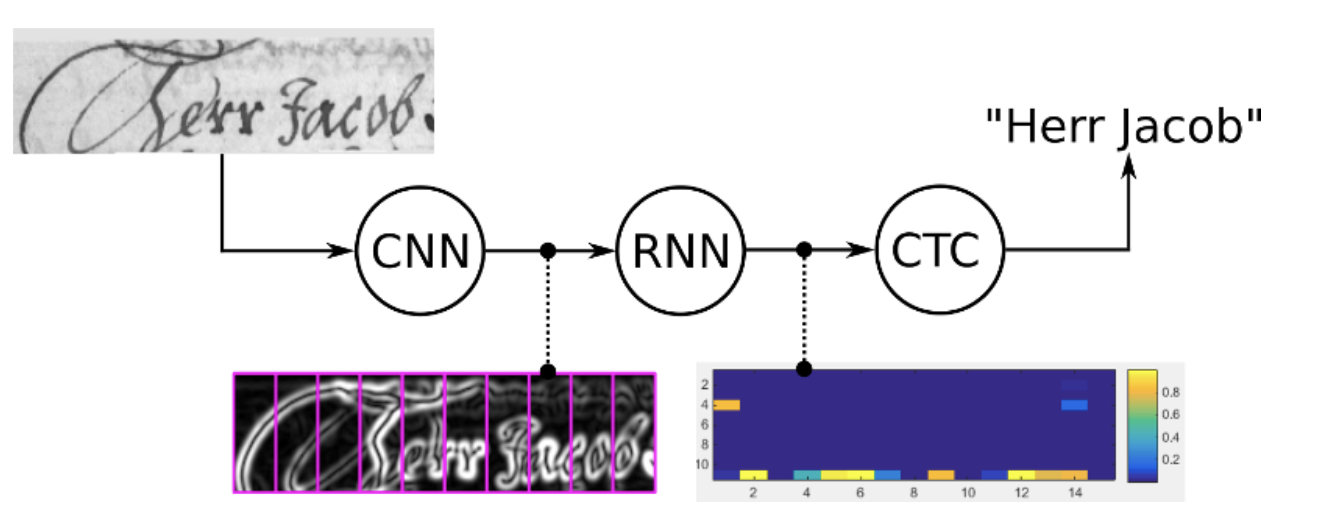
\includegraphics[width=150mm]{figures/image3.png}
\end{figure}

The NN-training will be guided by the CTC loss function. We only feed the output matrix of the NN and the corresponding ground-truth (GT) text to the CTC loss function.

\section{Post Processing}
Post-handling stage is the last phase of the proposed recognition framework. The post processing phase includes the conversion of the UNICODE in to standard output into any standard text encoding scheme.

\begin{figure}[H]
    \centering
    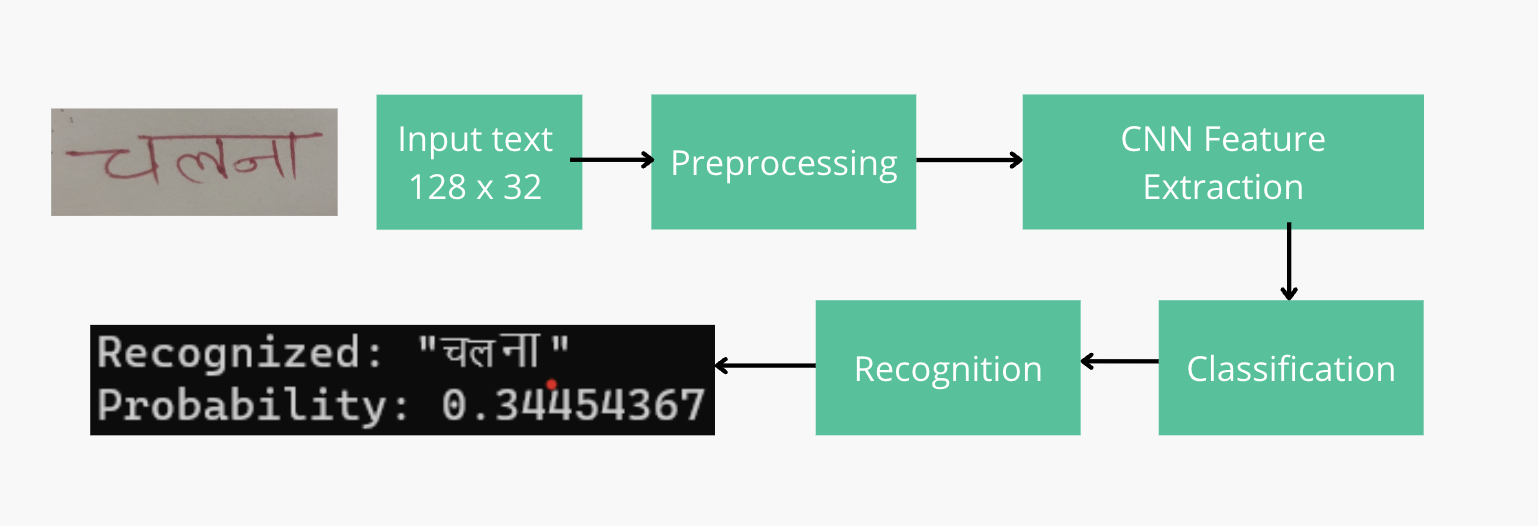
\includegraphics[width=150mm]{figures/image4.png}
    \caption{The Complete process of an OCR}
\end{figure}

%-----------------------------------------
% References/ Bibliography
%-----------------------------------------

\newpage

\label{chap:bib}
\section{Bibliography}

\begin{enumerate}

\item D. Yadav, S. Sanchez-Cuadrado, and J. Morato, “Optical Character Recognition for Hindi Language Using a Neural-network Approach,” Journal of Information Processing Systems, vol. 9, no. 1, pp. 117–140, Mar. 2013.

\item K. Dutta, P. Krishnan, M. Mathew and C. V. Jawahar, "Towards Spotting and Recognition of Handwritten Words in Indic Scripts," 2018 16th International Conference on Frontiers in Handwriting Recognition (ICFHR), 2018, pp. 32-37, doi: 10.1109/ICFHR-2018.2018.00015.

\item Nafiz Arica , Student Member , Fatos T. Yarman-vural , Senior Member, "Optical Character Recognition for Cursive Handwriting", IEEE TRANSACTIONS ON PATTERN ANALYSIS AND MACHINE INTELLIGENCE, VOL. 24, NO. 6, JUNE 2002

\item Gunna, S., Saluja, R., Jawahar, C.V. (2021). Transfer Learning for Scene Text Recognition in Indian Languages. In: Barney Smith, E.H., Pal, U. (eds) Document Analysis and Recognition – ICDAR 2021 Workshops. ICDAR 2021. Lecture Notes in Computer Science(), vol 12916. Springer, Cham.

\item Abhishek Mehta, Dr. Subhashchdra Desai, Dr. Ashish Chaturvedi, 2021, Hindi Handwritten Character Recognition from Digital Image using Deep Learning Neural Network, INTERNATIONAL JOURNAL OF ENGINEERING RESEARCH & TECHNOLOGY (IJERT) ICRADL – 2021 (Volume 09 – Issue 05)

\item Nisha Goyal1 , Er. Shilpa Jain, "Optimized Hindi Script Recognition using OCR Feature Extraction Technique", International Journal of Advanced Research in Computer and Communication Engineering Vol. 4, Issue 8, August 2015.

\item Bairagi, Prasanta Pratim. “Optical Character Recognition for Hindi.” (2018).

\end{enumerate}
\end{document} 
